%%%%%%%%%%%%%%%%%%%%%%%%%%%%%%%%%%%%%%%%%%%%%%%%%%%%%%%%%%%%%%%%%%%%%%%%%%%%%%%%
%%%%%%%%%%%%%%%%%%%%%%%%%%%%%%%%%%%%%%%%%%%%%%%%%%%%%%%%%%%%%%%%%%%%%%%%%%%%%%%%
%\documentclass[addpoints,12pt,solution]{exam}
\documentclass[preprint,12pt]{elsarticle}
%% Use the option review to obtain double line spacing

%% Use the options 1p,twocolumn; 3p; 3p,twocolumn; 5p; or 5p,twocolumn
%% for a journal layout:
%% \documentclass[final,1p,times]{elsarticle}
%% \documentclass[final,1p,times,twocolumn]{elsarticle}
%% \documentclass[final,3p,times]{elsarticle}
%% \documentclass[final,3p,times,twocolumn]{elsarticle}
%% \documentclass[final,5p,times]{elsarticle}
%% \documentclass[final,5p,times,twocolumn]{elsarticle}

%% The graphicx package provides the includegraphics command.
\usepackage{graphicx}
%% The amssymb package provides various useful mathematical symbols
\usepackage{amssymb}
\usepackage{amsmath}
\usepackage{titlesec}
\usepackage{breqn}
\usepackage{chemfig}
\usepackage{csvsimple}
\usepackage{tfrupee}  
%% The amsthm package provides extended theorem environments
%% \usepackage{amsthm}

%% The lineno packages adds line numbers. Start line numbering with
%% \begin{linenumbers}, end it with \end{linenumbers}. Or switch it on
%% for the whole article with \linenumbers after \end{frontmatter}.
\usepackage{lineno}
\usepackage{natbib}
\usepackage{hyperref}
% \usepackage[top=0.75in, bottom=0.75in, left=0.55in, right=0.85in]{geometry}
\usepackage{graphicx}
\usepackage{url}
\usepackage{palatino}
\usepackage{tabularx}
\usepackage{graphicx}
\usepackage{multicol}
\usepackage{graphicx}
\usepackage{amssymb}
\usepackage{float}
\usepackage{amsmath}
\usepackage{rotating}
\usepackage{subfigure}
\usepackage{multirow}
\usepackage{mathrsfs}
\usepackage{xfrac}
\usepackage[font=small,skip=0pt]{caption}
%\usepackage[numbers,sort&compress]{natbib}
%\usepackage{hyperref}
\usepackage{pgf,tikz}
\usetikzlibrary{shapes,arrows,chains}
\usetikzlibrary[calc]
\usepackage{graphicx}
\graphicspath{ {./images/}}
\usepackage{geometry}
\geometry{lmargin=1in,rmargin=1in,tmargin=1in,bmargin=1in}
\usepackage{lipsum}
%\pagestyle{empty}
\usepackage{natbib}
\pagenumbering{arabic}
%\usepackage[T1]{fontenc}
\usepackage{setspace}
\usepackage{mathptmx}
\usepackage{t1enc}
%\usepackage{xkeyval}
%\usepackage{chemformula}
%\usepackage{array}
%\usepackage{booktabs}
%\usepackage{hypdoc}
%\usepackage{listings}
%\usepackage{lmodern}
%\usepackage{mathpazo}
%\usepackage{microtype}
\usepackage{graphicx}
\usepackage{amssymb}
\usepackage{float}
\usepackage{amsmath}
\usepackage{rotating}
\usepackage{subfigure}
\usepackage{multirow}
\usepackage{xfrac}
\usepackage[font=small,skip=0pt]{caption}
%\usepackage[numbers,sort&compress]{natbib}
%\usepackage{hyperref}
\usepackage{pgf,tikz}
\usetikzlibrary{shapes,arrows,chains}
\usetikzlibrary[calc]
\usepackage{graphicx}
\usepackage{geometry}
\geometry{lmargin=1in,rmargin=1in,tmargin=1in,bmargin=1in}
\usepackage{lipsum}
%\pagestyle{empty}
\usepackage{natbib}
\pagenumbering{arabic}
%\usepackage[T1]{fontenc}
\usepackage{setspace}
\usepackage{mathptmx}
\usepackage{t1enc}
%\usepackage{xkeyval}
%\usepackage{chemformula}
%\usepackage{array}
%\usepackage{booktabs}
%\usepackage{hypdoc}
%\usepackage{listings}
%\usepackage{lmodern}
%\usepackage{mathpazo}
%\usepackage{microtype}
\usepackage{lineno,hyperref}
\usepackage{multirow}
\usepackage{cancel}
\usepackage{url}
\usepackage[norule]{footmisc}
\usepackage[utf8]{inputenc}
\usepackage[english]{babel}
\hypersetup{colorlinks = true,linkcolor = blue,urlcolor = blue}
% \fontfamily{SansSerif}
% \selectfont
% \usepackage[T1]{fontenc}
% \usepackage
%% natbib.sty is loaded by default. However, natbib options can be
%% provided with \biboptions{...} command. Following options are
%% valid:
%%   round  -  round parentheses are used (default)
%%   square -  square brackets are used   [option]
%%   curly  -  curly braces are used      {option}
%%   angle  -  angle brackets are used    <option>
%%   semicolon  -  multiple citations separated by semi-colon
%%   colon  - same as semicolon, an earlier confusion
%%   comma  -  separated by comma
%%   numbers-  selects numerical citations
%%   super  -  numerical citations as superscripts
%%   sort   -  sorts multiple citations according to order in ref. list
%%   sort&compress   -  like sort, but also compresses numerical citations
%%   compress - compresses without sorting
%%
%% \biboptions{comma,round}
% \biboptions{}
\usepackage{caption}
\usepackage{caption}
\usepackage{algorithm} 
\usepackage[noend]{algpseudocode}
\usepackage{amsmath}
\DeclareMathOperator*{\argmin}{argmin}
\DeclareMathOperator*{\argmax}{argmax}
\newcommand*{\argminl}{\argmin\limits}
\newcommand*{\argmaxl}{\argmax\limits}

\let\orupee\rupee
\def\rupee{\ifmmode\text{\orupee}\else\orupee\fi}


\begin{document}


\hrule
\vspace{1mm}
\noindent 
\begin{center}
{\Large MA5895 : Numerical Optimization} \\

{\large Combined Assignment Report} \\
{\large Cell Tower Problem   \hfill }
\end{center}
\vspace{1mm}
\noindent 


\titleformat{\section}
{\normalfont\fontfamily{phv}\fontsize{17}{20}\bfseries\itshape}{\thesubsection}{1em}{}

\titleformat{\subsection}
{\normalfont\fontfamily{phv}\fontsize{13}{17}\bfseries\itshape}{\thesubsection}{1em}{}

%%%%%%%%%%%%%%%%%%%%%%%%%%%%%%%%%%%%%%%%%%%%%%%%%%%%%%%%%%%%%%%%
% Enter name and roll number here
\noindent {\bf Name:} Pragnesh Rana \hfill {\bf Roll number:} ME17S301
%%%%%%%%%%%%%%%%%%%%%%%%%%%%%%%%%%%%%%%%%%%%%%%%%%%%%%%%%%%%%%%%%%
\vspace{2mm}
\hrule
\vspace{2mm}
{\small

\textbf{Summary : } The solution to find out the optimal location of cell tower sites is discussed here by keeping constrain over budget and population. To simulate the given problem, first random population is generated. The whole population is divided into regions using K-Means clustering. The centroid of each region is used as a potential site to plant to the cell tower. Out of all potential sites, the goal is to obtain the optimal locations such that total cost to plant the towers does not exceed the budget, and the maximum population is also served. The formulation is obtained by an instance of mixed-integer linear programming and solved by branch and bound technique using Gurobi's python based solver.  
}
\vspace{2mm}
\hrule

%%
%% Following citation commands can be used in the body text:
%% Usage of \cite is as follows:

%%   \cite{key}          ==>>  [#]
%%   \cite[chap. 2]{key} ==>>  [#, chap. 2]
%%   \citet{key}         ==>>  Author [#]

\tableofcontents

\section{Problem Statement}
In city planning, the issue is to find out optimal sites to plant the cell towers given the population and budget constraints. To solve the problem, divide the population into small regions based on the maximum capacity to plant the cell tower. Each site location may also cover other specified numbers of locations. Out of all possible cell tower sites, find out the optimal locations which can serve the maximum population keeping control over the budget.

\newpage

\section{Assumptions}
Assumed that,
\begin{itemize}
	\item The city is a rectangular region.
	
	    \item One region can be covered by more than one cell tower as they might have a different frequency.
	    
	    \item The cost of each tower is assumed as $30,00,000~\rupee$ \cite{cost} and other cost is 10$\%$ times the population(self+neighboring region) covered by each network.
	    
	    \item Each cellular location(centroid) can cover three neighbouring regions apart from covering its region. (Can be easily changed but in whole analysis kept fixed)
	    
	    \item The euclidean distance is used for measuring distance. 
	    
	    \item The resultant location of the cell site is average value of covered centroids (Average value of coordinates of centroid and its neighbouring centroid).
	
\end{itemize}


\section{Formulation} \label{sec:formulation}
Formulation of the problem is divided into two parts.
\begin{enumerate}
\item \textbf{Clusters of population data }

The population is divided into K-clusters using k-means algorithm given number potential cites to plant the cell towers. The partition is made in such way that each person is assigned with nearest possible mean location. Or generate K-clusters which minimizes the within-cluster sum of squares(variance).

The objective function for clustering is defined as\cite{wikiKmeans},

\begin{equation}
J = \argmin_s \sum_{i=1}^{k} \sum_{x\in s_i} ||x - \mu_i ||^2
\end{equation}

where,
\begin{itemize}
	\item $\mu_i$ = mean of points $s_i$
	\item $s$ = Population sets ${s_1,s_2,..,s_k} $
	\item k = Total required clusters
\end{itemize}

\item \textbf{Optimal location of sites}

After obtaining all the clusters, now objective is to find out the optimum locations which can cover maximum population keeping control over the budget. The formulation of problem is an instance of  mixed integer programming(MIP)\cite{maximal}.

The formulation is given as,
\begin{equation}
	\begin{aligned}
\text{Maximize} \hspace{2mm} Z &= \sum_{j \in R} p_j \cdot y_j \\
\text{S.T,} \hspace{3mm}\sum_{(i,j)} x_i &\geq y_j \hspace{3mm} \forall j \in \mathcal{R} \\
\sum_{i \in T} c_i \cdot x_i &\leq \text{Budget}
\end{aligned}
\end{equation}

where,
\begin{itemize}
	\item j - Index of regions $\in R$
	\item i - Index of optimal sites to build tower $\in T$
	\item T - Set of potential sites
	\item R - Set of regions
	\item $c_i$ - Cost of setting up a tower at site-i
	\item $p_j$ - Population at region-j
	\item $y_j$ - Binary variable for assignment of region \{1 if region is covered else 0\}
	\item $x_i$ - Binary variable for tower  \{1 if tower  is build else 0\}
\end{itemize}

\subitem \textbf{In Words:}
The objective function is to maximize the total covered population constraining over region and budget. The first constrain denotes that all location should be covered by at least one tower. Following, constrain denotes that total cost should not exceed the budget.
\end{enumerate}




The MIP(Mixd Interger Programming) problem is solved by linear-programming based branch-and-bound algorithm\cite{gurobiSol}. The solution is implemented using Gurobi (academic version) python based library\cite{gurobi}.  


 
\section{Approach to solve the problem with example}

\begin{itemize}
	\item In a specified rectangular region, using the limit of the region, population is generated by five blobs with appropriate $sigma$ such that spread is enough to cover enough region and 30$\%$ of the population is obtained by random spread over a given region.
	\item In Fundamental of cellular network\cite{david} it was mentioned that cellular network region could be approximated by hexagon so, the whole population is divided into given small number of regions(cluster) using k-means algorithm which follows the shape of a polygon(Approximation of pentagon or hexagon.)
	\item It was also mentioned that tower near to each other does not have the same frequency so, an overlap of frequency in one region may not be an issue\cite{david}. In a simulation, the tower located at the centroid of one region can cover three(or specified) nearest regions.
	
	\item Once all the regions is obtained, the centroid of each region denotes potential site to plant the cell tower.
	
	\item Out of all potential cites the optimal sites are obtained such that it can cover the maximum population given budget constrain.
	
	\item This problem is another example of maximal covering location problem\cite{maximal}and set cover problem. The mathematical formulation of the problem is given in section-\ref{sec:formulation} in the form of Mixed Integer Programming(MIP).
	
	\item The solution of the problem is obtained by Gurobi Optimizer python-based package. Further detail is given in section-\ref{sec:formulation}.
	
	\item Let's take an example,
	Input:
	\subitem Total Population = 1,30,000
	\subitem Count of Covering Region = 4 (self+3 Neighbor)
	\subitem Maximum Capacity to Plant Towers or Total regions = 12 
	\subitem Cost per each tower = $30,00,000~\rupee$
	\subitem Total budget = 10,00,000 * MAX Capacity + 10\% Total Population = $1,20,13,000~\rupee$
	
	\item Whole population is divided into 12 clusters as given in fig.-\ref{vor12}. Each cluster centroid is a potential site for the final cell location. However, the goal is to find out the optimal location of sites with specified constrains \ref{eq:constrain}. Problem is solved using gurobi solver which works based on maximum covering location algorithm with mixed integer programming. 
	

	
		The obtained result by running the simulation using aforementioned parameters is given below,
		
		\begin{figure}[H]
			\centering  
			\subfigure[Voronoi Diagram]
			{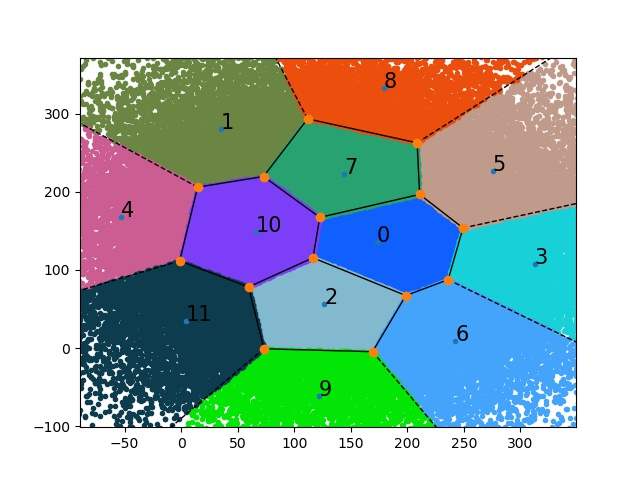
\includegraphics[width=0.43\linewidth]{./12Regions.jpg}\label{vor12}}
			\subfigure[Final cites to plant towers]
			{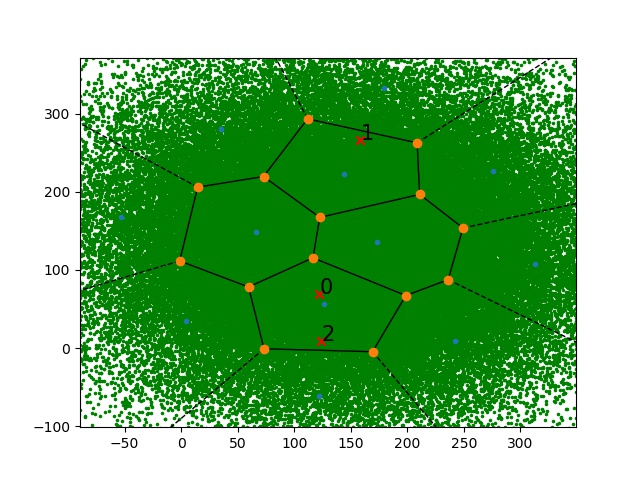
\includegraphics[width=0.43\linewidth]{./12FinalResult.jpg}\label{cites12}}
			\caption{Fig.-\ref{vor12} shows voronoi diagram obtained by diving the whole population into cluster using K-Means algorithm and Fig.-\ref{cites12} shows the final cites to plant the towers (By RED MARKED DOTS).}
			\label{fig:for12}
		\end{figure}
		
		\begin{table}[H]
			\centering
			\scalebox{0.61}{
				\begin{tabular}{|l|l|l|l|l|l|l|l|l|l|l|l|l|l|}
					\hline
					\textbf{Region} & 0 & 1 & 2 & 3 & 4 & 5 & 6 & 7 & 8 & 9 & 10 & 11 & \textbf{Total} \\ \hline
					\textbf{Population} & 44369 & 6539 & 11246 & 7466 & 4998 & 7909 & 8601 & 10757 & 4503 & 4743 & 12511 & 6898 & 130000 \\ \hline
					\textbf{Cost to build ($\rupee $)} & 3034514 & 3028266 & 3061623 & 3060339 & 3025948 & 3062592 & 3023455 & 3061383 & 3025205 & 3026205 & 3066372 & 3028755 & 30418113 \\ \hline
					\multicolumn{13}{|r|}{\textbf{Budget($\rupee $)}} & 12013000 \\ \hline
				\end{tabular}
		}
		\vspace{1mm}
		\caption{Summary of population and cost associated with each region along with available budget. }
		\label{tab:summary}
		\end{table}
		
			\begin{table}[H]
				\centering
				\begin{tabular}{|c|c|c|c|}
					\hline
					\textbf{RegionCenter} & \textbf{NeighborCenter0} & \textbf{NeighborCenter1} & \textbf{NeighborCenter2} \\ \hline
					0 & 7 & 2 & 10 \\ \hline
					1 & 7 & 10 & 4 \\ \hline
					2 & 0 & 10 & 9 \\ \hline
					3 & 6 & 5 & 0 \\ \hline
					4 & 10 & 1 & 11 \\ \hline
					5 & 3 & 7 & 0 \\ \hline
					6 & 3 & 2 & 9 \\ \hline
					7 & 0 & 10 & 8 \\ \hline
					8 & 7 & 5 & 1 \\ \hline
					9 & 2 & 6 & 11 \\ \hline
					10 & 0 & 7 & 2 \\ \hline
					11 & 2 & 10 & 4 \\ \hline
				\end{tabular}					\vspace{1mm}
				\caption{Table of centroid and its three nearest centroid index}
				\label{tab:centeroids}
			\end{table}
		
	\item Centroid and its three nearest neighbor centroids are given in table-\ref{tab:centeroids} which indicates if cell tower is planted on specific region center, it can also cover three nearest regions along with its region. The objective is to find out the best possible sites which can cover maximum population with restriction of budget. For example if cell tower is planted at centroid location-0 then it can cover regions with centroid location 7, 2, and 10,which can be verified from figure-\ref{vor12}.
	
	\item The problem is solved by running the algorithm considering specified constrain. Obtained result is given in fig-\ref{cites12}. The centroid 2,8 and 9 are resultant place obtained by algorithm.
	
	\item The tower at centroid location-2 can cover region 2,0,10,9. Likewise, tower at location 8 and 9 also covers the regions 8,7,5,1 and 9,2,6,11.
	
	\item Final location of cell site is obtained by taking average value coordinates of centroids, as location 2 can cover regions-2,0,10 and 9.
	
	\item It is observed that the region 2 and 9 are covered twice. The region 4 and 3 are not covered due to budget constrain.
	
	\item Overall, to cover 86.95\% population, 75.94\% budget is utilized.
\end{itemize}

\newpage

\section{Implemented algorithm procedure}\label{sec:algo}
	\begin{algorithm}[H]
		\caption{ To find out optimal cell tower location}\label{alg:algo}
		\begin{algorithmic}[1]
			%%				  				\\\hrulefill
			
			\State $population$: Size of the population		
			\State $NOB$: Number of Blobs
			\State $NOC$: Number of Clusters based on capacity to plant towers
			\State $DistBtnCentroidNNeighbor$ : Calculates distance of each centroid to all other centroids
			\Procedure{GeneratePopulation}{population,NOB}  
			\vspace{1mm} \Comment{To generate artificial Data}
			\State BlobPopulation = Generate blobs(NOB)  \Comment{Used scikit learn}
			\State RandomPopulation = Generate data points in specified limit \Comment{random function}
			\State TotalPopulationData = BlobPopulation + RandomPopulation 
			\State \Return TotalPopulationData
			\EndProcedure
			\vspace{1mm}
			
			\Procedure{GenerateClusters}{TotalPopulationData,NOC}
			\State labels , ClusterCentroid = KMEAN(TotalPopulationData,NOC) \Comment{scikit's kmean algo}
			\State \Return labels, ClusterCentroid
			\EndProcedure					\vspace{1mm}
			
			
			\Procedure{DistBtnCentroidNNeighbor}{ClusterCentroid}
			\State AllocatedFacilityData = Empty \Comment{To store index of nearest specified neighbors}
			\For{ClusterCentroid} 
				\State Dist = find Distance from all centroids(ClusterCentroid) \Comment{Euclidean distance}		
				\State AllocatedFacilityData.append($\argmin(Dist)[1:4]$) 	\Comment{Specified neighbors, Here 3}
			\EndFor
			\State \Return AllocatedFacilityData
			\EndProcedure
		\vspace{1mm}			
		
		\Procedure{CellTowerProblem}{AllocatedFacilityData,RegionWisePopulation}
		\State \Call{Gurobi API}{ }
		\State Obj = Define Objecive Function to cover maximum population
		\State C1= Define Constrain to cover whole population 
		\State C2= Define Constrain for Budget 
		\State OptimizedLocations = Run API(Obj, C1, C2)
		\State \Return OptimizedLocations
		\EndProcedure
		
		\vspace{1mm}
		\Procedure{FinalLocations}{OptimizedLocation,ClusterCentroid,AllocatedFacilityData}
		\State FinalLocations = Empty \Comment{Array}
		\For{OptimizedLocation}
		\State FinalLocations.append(average(AllocatedFacilityData[OptimizedLocation]))
		\EndFor
		\State \Return FinalLocations
		\EndProcedure
		
		\vspace{1mm}
		\Procedure{Simulate}{ }
		\State TotalPopulationData = \Call{GeneratePopulation}{population,NOB}  
		\State labels, ClusterCentroid = \Call{GenerateClusters}{TotalPopulationData,NOC}
		\State \Call{VoronoiDiagram}{ClusterCentroid}
		\State RegionWisePopulation = \Call{SeperateDataByLabel}{labels,TotalPopulationData}
		\State AllocatedFacilityData = \Call {DistBtnCentroidNNeighbor}{ClusterCentroid}
		\State OptimizedLocations =\Call{CellTowerProblem}{AllocatedFacilityData,RegionWisePopulation}
		\State FinalLocations = \Call{FinalLocations}{OptimizedLocation,ClusterCentroid,AllocatedFacilityData}
		\EndProcedure
		\end{algorithmic}
	\end{algorithm}
	

\section{Results}

\subsection{Result with few values of input}

\begin{itemize}
	
\item \textbf{Case:1}

Input:
\subitem Total Population = 1,30,000
\subitem Count of Covering Region = 4 (self+3 Neighbor)
\subitem Maximum Capacity to Plant Towers or Total regions = 12 
\subitem Cost per each tower = $30,00,000~\rupee$
\subitem Total budget = 10,00,000 * MAX Capacity + 10\% Total Population = $1,20,13,000~\rupee$

	\begin{figure}[H]
		\centering  
		\subfigure[Voronoi Diagram]
		{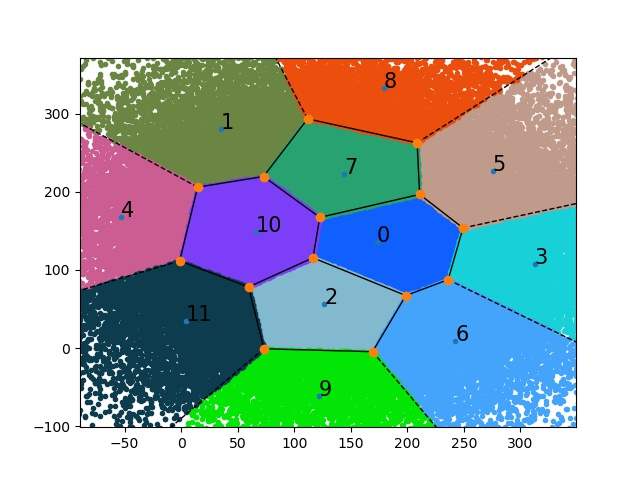
\includegraphics[width=0.43\linewidth]{./12Regions.jpg}\label{vor12_}}
		\subfigure[Final cites to plant towers]
		{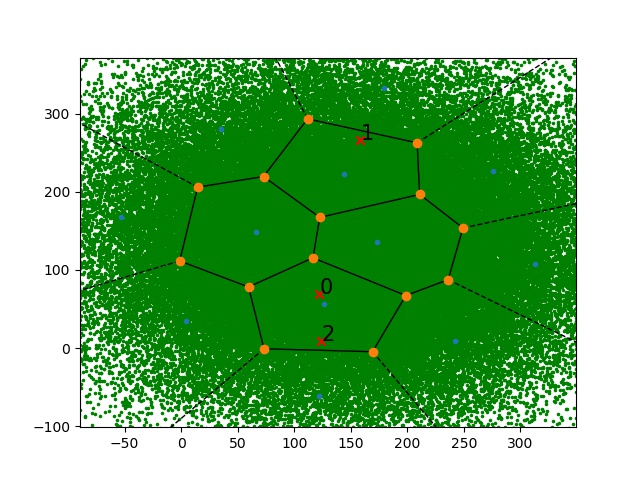
\includegraphics[width=0.43\linewidth]{./12FinalResult.jpg}\label{cites12_}}
		\caption{Fig.-\ref{vor12_} shows voronoi diagram obtained by diving the whole population into cluster using K-Means algorithm and Fig.-\ref{cites12_} shows the final cites to plant the towers (By RED MARKED DOTS).}
		\label{fig:for12_}
	\end{figure}

The locations to plant cell towers are obtained by average value of region shown in fig.-\ref{vor12_} marked by centroid 2,8,9 and its 3 neighboring regions. Final Location is given in fig-\ref{cites12_} by red dots. \textbf{To cover 86.95\% of population 75.94\% budget is utilized.} 

\item \textbf{Case:2}

Input:
\subitem Total Population = 1,30,000
\subitem Count of Covering Region = 4 (self+3 Neighbor)
\textbf{\subitem Maximum Capacity to Plant Towers or Total regions = 25}
\subitem Cost per each tower = $30,00,000~\rupee$
\subitem Total budget = 10,00,000 * MAX Capacity + 10\% Total Population = $2,50,13,000~\rupee$
	\begin{figure}[H]
		\centering  
		\subfigure[Voronoi Diagram]
		{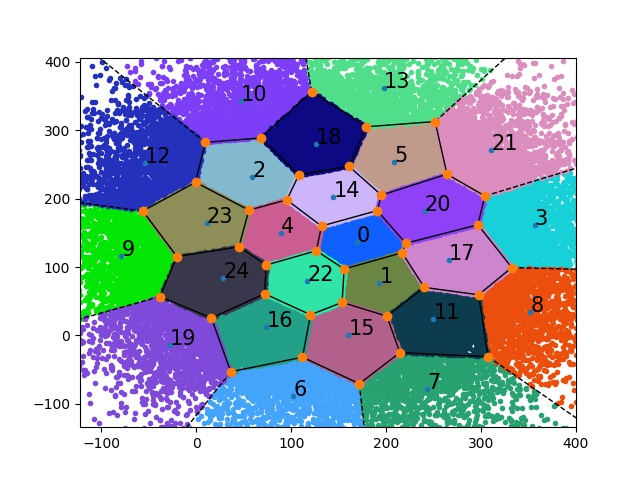
\includegraphics[width=0.43\linewidth]{./25Regions.jpg}\label{vor25}}
		\subfigure[Final cites to plant towers]
		{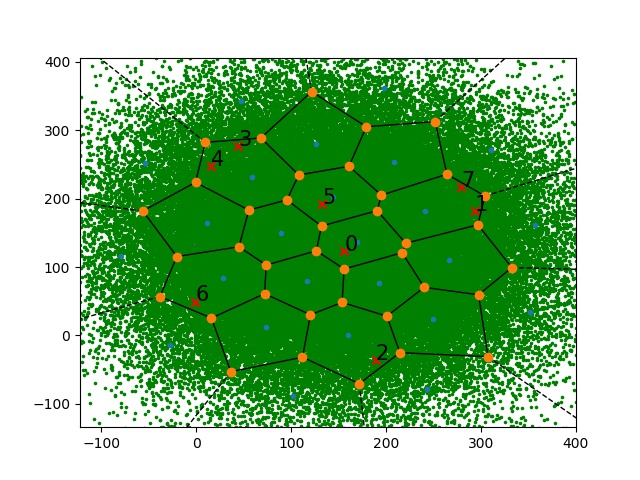
\includegraphics[width=0.43\linewidth]{./25FinalResult.jpg}\label{cites25}}
		\caption{Fig.-\ref{vor25} shows voronoi diagram obtained by diving the whole population into cluster using K-Means algorithm and Fig.-\ref{cites25} shows the final cites to plant the towers (By RED MARKED DOTS).}
		\label{fig:for25}
	\end{figure}

The locations to plant cell towers are obtained by average value of region shown in fig.-\ref{vor25} marked by centroid 0,3,7,10,12,14,19,21 and its 3 neighboring regions. Final 8 location is given in fig-\ref{cites25} by red dots. \textbf{To cover 94.55\% of population 96.55\% budget is utilized. }

\item \textbf{Case:3}

Input:
\subitem Total Population = 1,30,000
\subitem Count of Covering Region = 4 (self+3 Neighbor)
\textbf{\subitem Maximum Capacity to Plant Towers or Total regions = 50} 
\subitem Cost per each tower = $30,00,000~\rupee$
\subitem Total budget = 10,00,000 * MAX Capacity + 10\% Total Population = $5,20,13,000~\rupee$
	\begin{figure}[H]
		\centering  
		\subfigure[Voronoi Diagram]
		{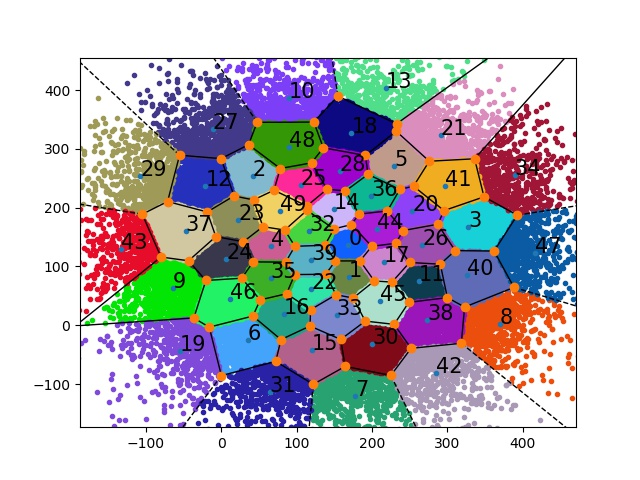
\includegraphics[width=0.43\linewidth]{./50Regions.jpg}\label{vor50}}
		\subfigure[Final sites to plant towers]
		{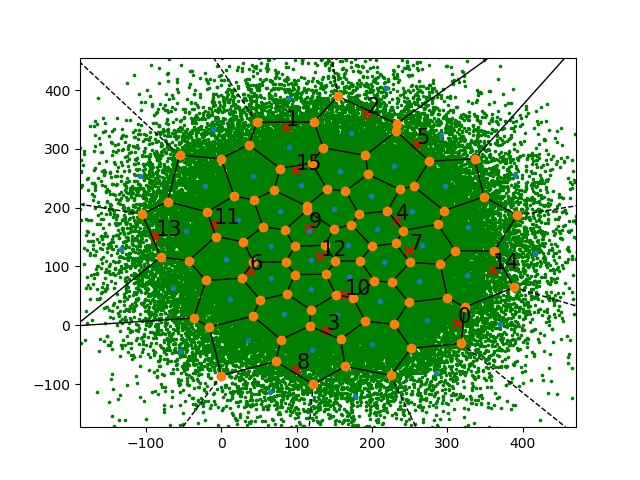
\includegraphics[width=0.43\linewidth]{./50FinalResult.jpg}\label{cites50}}
		\caption{Fig.-\ref{vor50} shows voronoi diagram obtained by diving the whole population into cluster using K-Means algorithm and Fig.-\ref{cites50} shows the final sites to plant the towers (By RED MARKED DOTS).}
		\label{fig:for50}
	\end{figure}

The locations to plant cell towers are obtained by average value of region shown in fig.-\ref{vor25} marked by centroid 8,10,13,15,20,21,24,26,31,32,33,37,39,43,47,48 and its 3 neighboring regions. Final 16 locations are given in fig-\ref{cites25} by red dots. \textbf{To cover 97.73\% of population 96.27\% budget is utilized. }

	
\item\textbf{ Case:4}

Input:
\subitem \textbf{Total Population = 50,000}
\subitem Count of Covering Region = 4 (self+3 Neighbor)
\subitem Maximum Capacity to Plant Towers or Total regions = 25 
\subitem Cost per each tower = $30,00,000~\rupee$
\subitem Total budget = 10,00,000 * MAX Capacity + 10\% Total Population = $2,50,05,000~\rupee$
	\begin{figure}[H]
		\centering  
		\subfigure[Voronoi Diagram]
		{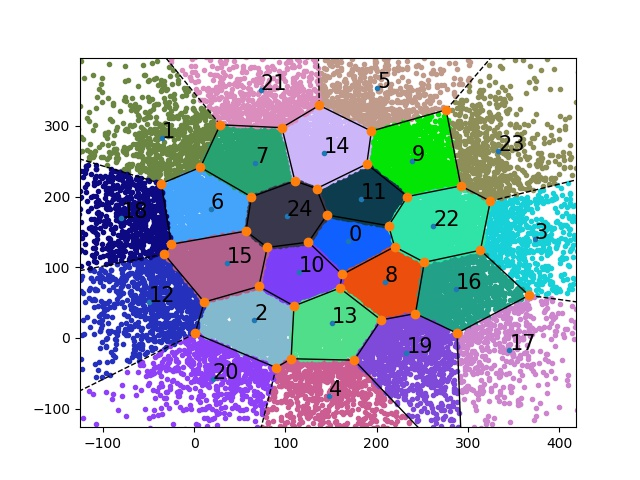
\includegraphics[width=0.43\linewidth]{./25_50_Regions.jpg}\label{vor_25_50}}
		\subfigure[Final sites to plant towers]
		{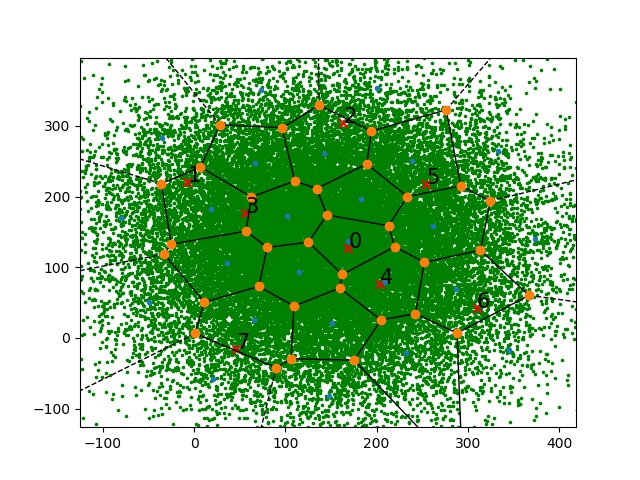
\includegraphics[width=0.43\linewidth]{./25_50_FinalResult.jpg}\label{cites_25_50}}
		\caption{Fig.-\ref{vor_25_50} shows voronoi diagram obtained by diving the whole population into cluster using K-Means algorithm and Fig.-\ref{cites_25_50} shows the final sites to plant the towers (By RED MARKED DOTS).}
		\label{fig:for_25_50}
	\end{figure}
	
The locations to plant cell towers are obtained by average value of region shown in fig.-\ref{vor_25_50} marked by centroid 0,1,5,6,8,9,17,20 and its 3 neighboring regions. Final 16 locations are given in fig-\ref{cites_25_50} by red dots. \textbf{To cover 94.86\% of population 96.21\% budget is utilized.} 

\item \textbf{Case:5}

Input:
\subitem Total Population = 50,000
\subitem \textbf{Count of Covering Region = 5 (self+3 Neighbor)}
\subitem Maximum Capacity to Plant Towers or Total regions = 25 
\subitem Cost per each tower = $30,00,000~\rupee$
\subitem Total budget = 5,00,000 * MAX Capacity + 10\% Total Population = $2,50,05,000~\rupee$
	\begin{figure}[H]
		\centering  
		\subfigure[Voronoi Diagram]
		{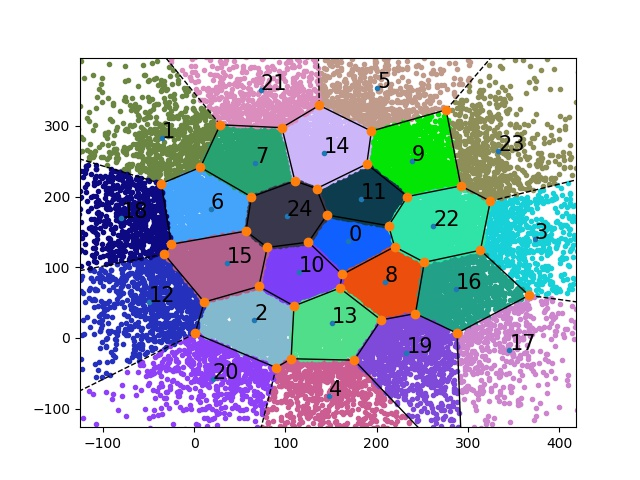
\includegraphics[width=0.43\linewidth]{./25_50_5_Regions.jpg}\label{vor_25_50_5}}
		\subfigure[Final sites to plant towers]
		{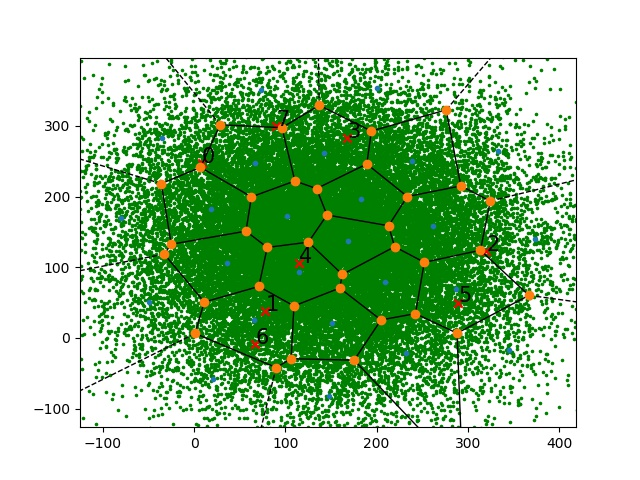
\includegraphics[width=0.43\linewidth]{./25_50_5_FinalResult.jpg}\label{cites_25_50_5}}
		\caption{Fig.-\ref{vor_25_50_5} shows voronoi diagram obtained by diving the whole population into cluster using K-Means algorithm and Fig.-\ref{cites_25_50_5} shows the final sites to plant the towers (By RED MARKED DOTS).}
		\label{fig:for25_50_5}
	\end{figure}

The locations to plant cell towers are obtained by average value of region shown in fig.-\ref{vor_25_50_5} marked by centroid 1,2,3,5,10,17,20,21 and its 4 neighboring regions. Final 16 locations are given in fig-\ref{cites_25_50_5} by red dots. \textbf{To cover 100\% of population 96.24\% budget is utilized.} 


\item \textbf{Case:6}

Input:
\subitem Total Population = 50,000
\subitem \textbf{Count of Covering Region = 4 (self+3 Neighbor)}
\subitem Maximum Capacity to Plant Towers or Total regions = 25 
\textbf{\subitem Cost per each tower = $2,00,000~\rupee$
\subitem Total budget = 1,00,000 * MAX Capacity + 10\% Total Population = $25,05,000~\rupee$}
\begin{figure}[H]
	\centering  
	\subfigure[Voronoi Diagram]
	{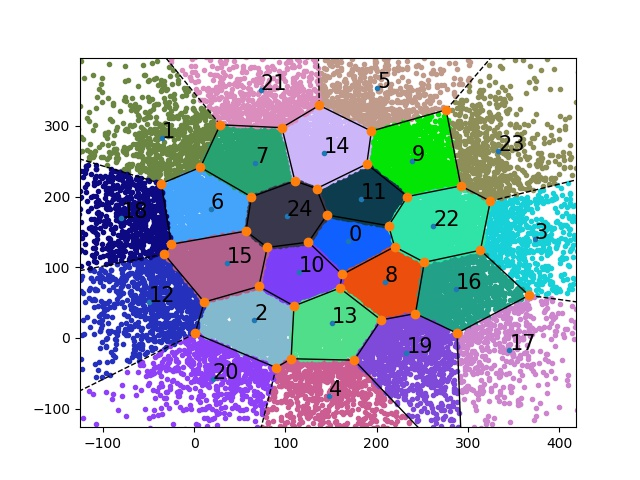
\includegraphics[width=0.43\linewidth]{./25_4_Regions.jpg}\label{vor_25_4}}
	\subfigure[Final sites to plant towers]
	{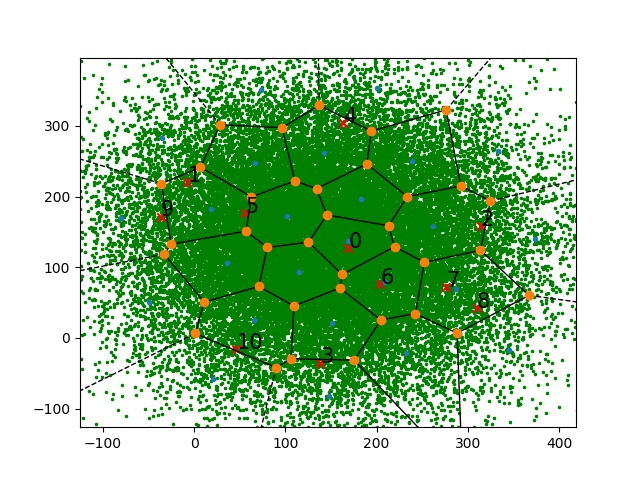
\includegraphics[width=0.43\linewidth]{./25_4_FinalResult.jpg}\label{cites_25_4}}
	\caption{Fig.-\ref{vor_25_4} shows voronoi diagram obtained by diving the whole population into cluster using K-Means algorithm and Fig.-\ref{cites_25_4} shows the final sites to plant the towers (By RED MARKED DOTS).}
	\label{fig:for25_4}
\end{figure}

The locations to plant cell towers are obtained by average value of region shown in fig.-\ref{vor_25_4} marked by centroid 0,1,3,4,5,6,8,16,17,18,20 and its 3 neighboring regions. Final 16 locations are given in fig-\ref{cites_25_4} by red dots. \textbf{To cover 98.54\% of population 90.53\% budget is utilized.} 

\end{itemize}

\subsection{Largest problem size you can solve}
Tried to solve problem for region-size of 10,000(clusters). But got(laptop doesn't have space),\\ MemoryError: Unable to allocate 9.69 GiB for an array with shape (130000, 10000) and data type float64.\\
The maximum I tried  till 1000 clusters. The computational complexity is discussed in next section. Based on computational complexity largest problem size can be determined.

\subsection{Computational time as a function of input parameters}
Out of all input parameters, the major affecting parameter which can affect the computational cost is number of region. As number of region is directly related to matrix size. The computational time mentioned is only measured between time taken to find out final centroid location. Basically, time taken to solve Mixed Integer Programming. The result is given in fig.-\ref{fig:time}.

\begin{figure}[H]
	\centering  
	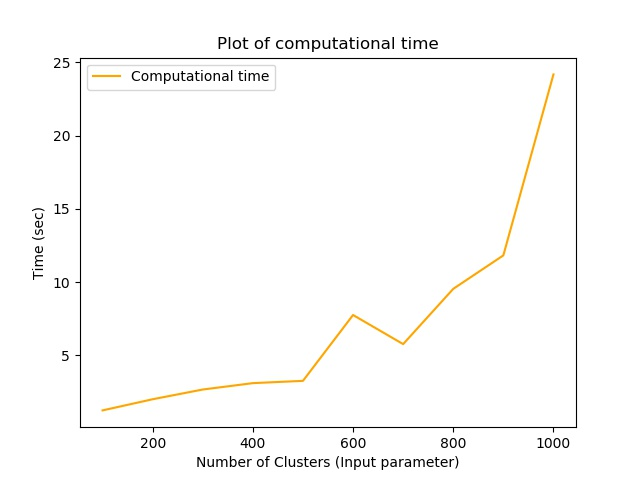
\includegraphics[width=0.8\linewidth]{./time.jpg}
	\vspace{2mm}
	\caption{Plot of Computational Complexity (loglog)}
	\label{fig:time}
\end{figure}

\textbf{ Why up \& downs in time?(Observation)} \\
 With change in number of regions(potencial sites), the orientation and shape of region also get changed. The gurobi solver uses branch and bound algorithm. Along with, it uses some heuristics, cutting plane methods and presolve techniques\cite{gurobiSol}. Due to change in orientation and shape of regions, the aforementioned techniques get affected computationally which may result in variation of time.



	\newpage
	
\section{References}
	%%
	%% Following citation commands can be used in the body text:
	%% Usage of \cite is as follows:
	
	%%   \cite{key}          ==>>  [#]
	%%   \cite[chap. 2]{key} ==>>  [#, chap. 2]
	%%   \citet{key}         ==>>  Author [#]
	
	%% References with bibTeX database:
	\bibliographystyle{ieeetr}
	\bibliography{biblio.bib}					
	%% Authors are advised to submit their bibtex database files. They are
	%% requested to list a bibtex style file in the manuscript if they do
	%% not want to use model1-num-names.bst.
	
	%% References without bibTeX database:
	
	% \begin{thebibliography}{00}
	
	%% \bibitem must have the following form:
	%%   \bibitem{key}...
	%%
	
	% \bibitem{}
	
	% \end{thebibliography}


\end{document}